\documentclass[10pt, reqno]{amsart}
\usepackage[margin = 0.5 in]{geometry}
\usepackage{multicol}
\usepackage{float}
\usepackage{fancyhdr}
\usepackage{graphicx}
\usepackage{hyperref}
\usepackage{fancyvrb}

\setlength{\abovecaptionskip}{5pt plus 3pt minus 3pt}

\hypersetup{colorlinks=true,allcolors=blue}
\pagestyle{fancy} \fancyhead{} \fancyfoot[C]{\normalsize\thepage}
\renewcommand{\headrulewidth}{0pt}
\begin{document}
\title{ME 5311 \quad Assignment 1 \quad Jacob Ivanov}

\maketitle

\begin{multicols}{2}
The Burning Ship fractal is described by the following iterative equation:
\begin{equation}
    z_{n + 1} = \Big( |\Re[z_n]|^2 + \mathbf{i} |\Im[z_n]| \Big)^2 - c
\end{equation}
A point $c$ is considered to be part of the Burning Ship Set if $\lim_{n \to \infty} [z_n]$ is bounded. A numerical algorithm was implemented in Julia that iterates Eq. (1) 200 times, and considered $|z_{200}| < 200$ to be part of the Burning Ship Set. The results of which are shown in Fig. 1 below, on the region $x \in [-2, +2]$ and $y \in [-2, +2]$:

\begin{figure}[H]
    \centering
    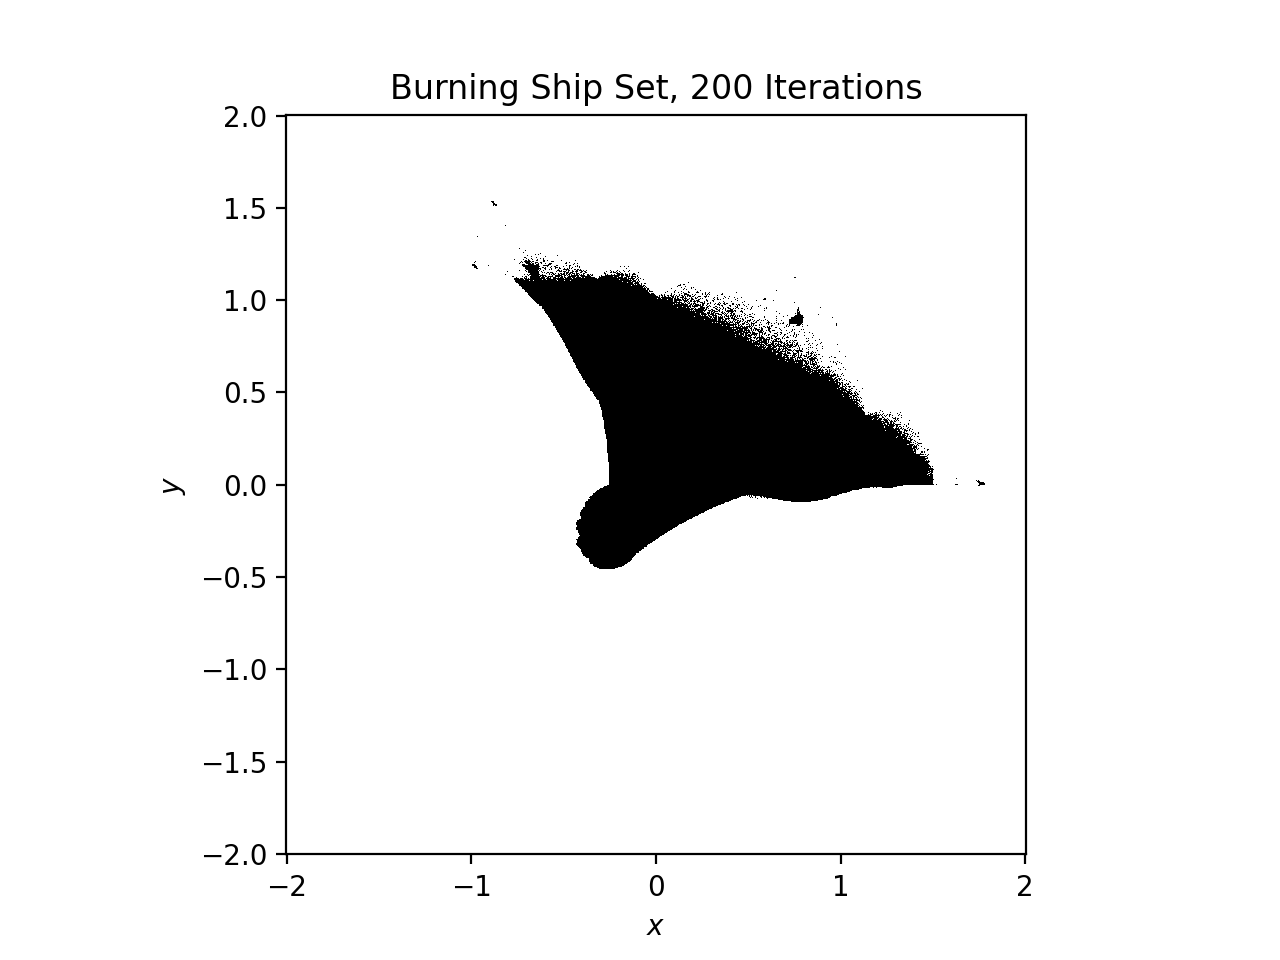
\includegraphics[width=1\linewidth]{burning_ship_set.png}
    \caption{Burning Ship Set, Region 1}
    \label{fig:1}
\end{figure}

However, this binary distinction makes for a rather uninteresting plot compared to showing the iteration at which $z_n$ is no longer bounded. Defining $c = x + \mathbf{i}y$, and a new function $N(c) = N(x + \mathbf{i}y) = n \, \mathrm{where} \, |z_n| > 200$, by taking the natural logarithm of this $n$, we obtain Fig. 2 below. 
\begin{figure}[H]
    \centering
    \includegraphics[width=1\linewidth]{burning_ship.png}
    \caption{Burning Ship Contour, Region 1}
    \label{fig:2}
\end{figure}

As a fractal, the structure is self-similar at any scale, which can be seen if we repeat this procedure on an arbitrary new region, in this case, $x \in [-1.25, -0.75]$ and $y \in [1.25, 1.75]$. 
\begin{figure}[H]
    \centering
    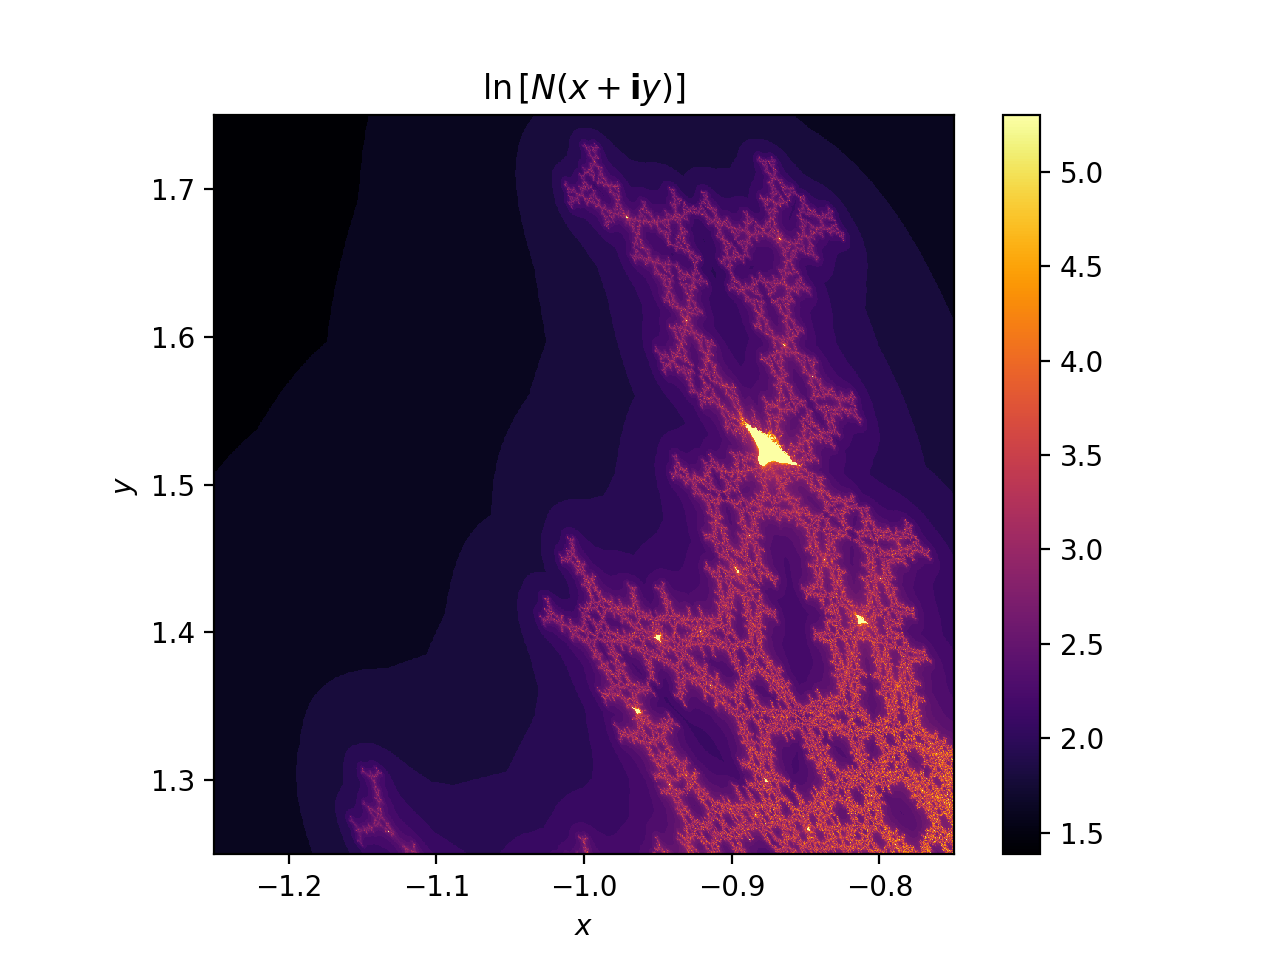
\includegraphics[width=1\linewidth]{burning_ship_zoom.png}
    \caption{Burning Ship Contour, Region 2}
    \label{fig:3}
\end{figure}

\section{Notes}
The assignment details encouraged concise code, specifically calling for $<$50 lines. Though the final product \texttt{burning\_ ship.jl} was 73 lines, where the main procedure is the first 50 lines, this was due to comments, and toggled sections to produce Fig. 1-3 above. Excluding these, the pre-plotting section is roughly 30 lines with reasonable spacing. 

One additional technical note is that Julia is column-major, whereas Python Numpy is row-major. As a result, where Julia passes the relevent array to \texttt{PyPlot.jl}, it is transposed.

\end{multicols}

\end{document}